% LaTeX source for book ``模形式初步'' in Chinese
% Copyright 2020  李文威 (Wen-Wei Li).
% Permission is granted to copy, distribute and/or modify this
% document under the terms of the Creative Commons
% Attribution 4.0 International (CC BY 4.0)
% http://creativecommons.org/licenses/by/4.0/

\chapter{维数公式与应用}
本章选定余有限 Fuchs 群 $\Gamma \subset \SL(2,\R)$. 一旦掌握模曲线 $X(\Gamma)$ 的几何, 可以在其上定义自然的线丛 $\bomega_\Gamma$, 使得级为 $\Gamma$ 而权为 $k$ 的模形式能够典范地等同于 $\bomega_\Gamma^{\otimes k}$ 的全纯截面; 事实上, $\bomega_\Gamma|_{Y(\Gamma)}$ 等于平凡线丛 $\mathcal{H} \times \CC \to \mathcal{H}$ 对 $\Gamma$ 作用 $(\tau, z) \xmapsto{\gamma} (\gamma\tau, j(\gamma, \tau)z)$ 的商, 在尖点处则需要适当的延拓. 详见之后的定理 \ref{prop:modular-vs-omega}.

此法美则美矣, 却有两个问题.
\begin{enumerate}
	\item 若 $\Gamma$ 有椭圆点, 则 $X(\Gamma)$ 必须视为叠而不只是 Riemann 曲面, 线丛和截面的概念都需要适度拓展, 导致理论包袱大增;
	\item 即使无椭圆点, 单有 $\bomega_\Gamma$ 的存在性也无助于计算 $M_k(\Gamma)$ 和 $S_k(\Gamma)$ 的维数.
\end{enumerate}

鉴于上述理由, 线丛 $\bomega_\Gamma$ 在无椭圆点情形的研究将留待 \S\ref{sec:cplx-viewpoint} 探讨. 本章直接通过典范线丛 $\Omega_{X(\Gamma)}$ 来研究偶数权模形式空间的维数公式, 容许 $\Gamma$ 有椭圆点. 线丛 $\bomega_\Gamma^{\otimes 2}$ 和 $\Omega_{X(\Gamma)}$ 之间有密切的联系, 称为小平--Spencer 同构, 一样留待 \S\ref{sec:cplx-viewpoint} 处理.

更详细地说, 我们将把权为 $2k$ 的模形式联系于 $\Omega_{X(\Gamma)}^{\otimes k}$ 的某些亚纯截面, 可能的极点由某个 $\Q$-除子 $D_\Gamma$ 控制. 当 $k$ 不太小时, 截面空间的维数可以倚靠 Riemann 曲面理论中的 Riemann--Roch 定理来计算, 相关推导需要关于基本区域的信息.

作为一则应用, 我们将在 \S\ref{sec:dimension-full} 为级为 $\SL(2,\Z)$ 的模形式空间确定其维数, 连带证明分次 $\CC$-代数 $M(1) := \bigoplus_k M_k(\SL(2,\Z))$ 由 Eisenstein 级数 $E_4, E_6$ 生成; 进一步, $E_4, E_6$ 在 $\CC$ 上代数无关, 其零点亦可完全确定 (命题 \ref{prop:zeros-E4-E6}), 而尖点形式空间 $\bigoplus_k S_k(\SL(2,\Z))$ 则可以用模判别式 $\Delta$ 表达为 $M(1)$ 的分次理想 $\Delta \cdot M(1)$. 这一特例有相对简单的论证, 见 \cite[Chapter VII]{Se73}.

奇数权情形也有类似的维数公式, 见 \S\ref{sec:dimension-formula-odd}; 关键是证明奇数权亚纯模形式的存在性 (定理 \ref{prop:existence-meromorphic-odd}).

研究维数的另一套工具是迹公式, 其应用范围更广, 但所需的计算也比较深入, 本书不予讨论; 读者可参考 \cite[\S 6]{Mi89}.

如无另外说明,所论的 Riemann 曲面都是连通的. 包括 Riemann--Roch 定理在内的相关背景知识可参阅附录 B. 文献 \cite[\S 3.9]{DS05} 和 \cite{Mi89} 附录含有更多的维数数据.

\section{热身: 除子类的计算}
考虑余有限 Fuchs 群 $\Gamma \subset \SL(2,\R)$. 定理 \ref{prop:Fuchsian-1st-kind} 和 \ref{prop:Fuchsian-1st-kind-pasting} 提供以下信息:
\begin{compactitem}
	\item 选定 $\Gamma$ 的非椭圆点 $x_0 \in \mathcal{H}$, 则 Dirichlet 区域 $D(x_0)$ 是测地多边形;
	\item $X(\Gamma)$ 是紧 Riemann 曲面;
	\item 尖点集 $X(\Gamma) \smallsetminus Y(\Gamma)$ 有限.
\end{compactitem}

\begin{convention}\label{conv:e}
	对任意 $\tau \in \mathcal{H}^*$, 命
	\[ e(\tau) := \begin{cases}
		\left| \overline{\Gamma}_\tau \right|, & \tau \in \mathcal{H} \\
		\infty, & \tau \in \mathcal{H}^* \smallsetminus \mathcal{H}.
	\end{cases}\]

	注意到 $\tau \in \mathcal{H}$ 为椭圆点等价于 $e(\tau) > 1$. 此量仅依赖于 $\tau$ 在 $X(\Gamma)$ 中的像 $x$, 故可记之为 $e(x)$.
\end{convention}

\begin{definition}\label{def:Hodge-class}
	\index[sym1]{$D_\Gamma$} \index[sym1]{$L_\Gamma$}
	定义 $X(\Gamma)$ 上的 $\Q$-除子
	\begin{align*}
		D_\Gamma & := \sum_{x \in X(\Gamma)} \left( 1 - \frac{1}{e(x)} \right) x \\
		& = \sum_{c: \text{尖点}} c + \sum_{y: \text{椭圆点的像}} \left( 1 - \frac{1}{e(y)} \right) y \; \in \Div(X(\Gamma))_{\Q} \\
	\end{align*}
	其中 $e(x)$ 如约定 \ref{conv:e}, 再定义 $\Q$-除子类
	\[ L_\Gamma := D_\Gamma + K_{X(\Gamma)} \; \in \Pic(X(\Gamma))_{\Q} . \]
\end{definition}

\begin{theorem}[见 \cite{Bea95} Corollary 10.4.4]\label{prop:D-estimate}
	令 $g = g(X(\Gamma))$ 表 $X(\Gamma)$ 的亏格, $\epsilon_\infty$ 表尖点个数, 那么相对于双曲度量,
	\begin{align*}
		\deg(L_\Gamma) & = 2g - 2 + \epsilon_\infty + \sum_{\substack{y \in Y(\Gamma): \\ \text{来自椭圆点}}} \left( 1 - \dfrac{1}{e(y)} \right) \\
		& = (2\pi)^{-1} \mes(Y(\Gamma)) \; > 0.
	\end{align*}
\end{theorem}
\begin{proof}
	由 $\deg K_{X(\Gamma)} = 2g - 2$ (注记 \ref{rem:RR}) 得到第一个等号. 关键在第二个等号. 向 $D(x_0)$ 添入它在 $\mathcal{H}^*$ 中的无穷远点以得到 $D(x_0)^*$. 于是 $\mes(Y(\Gamma)) = \mes(D(x_0))$, 而根据命题 \ref{prop:fundamental-domain-paste}, $X(\Gamma)$ 同胚于 $D(x_0)^*/\sim$, 其中 $\sim$ 是由 $(x \sim y) \iff (\exists \gamma \in \overline{\Gamma}, \; \gamma x = y)$ 定义的等价关系. 根据定理 \ref{prop:Fuchsian-1st-kind}, 这给出 $X(\Gamma)$ 的一个有限剖分, 由之可以计算 Euler 示性数等拓扑不变量.
	
	按定义 \ref{def:sides} 和注记 \ref{rem:side-pairing} 之法细分 $D(x_0)^*$ 的边, 可确保落在 $\partial D(x_0)^*$ 上的椭圆点都是顶点. 既然 $D(x_0)^*$ 边数已有限, 注记 \ref{rem:side-pairing} 已说明细分后边数仍有限, 于是 Euler 示性数 $\chi(X(\Gamma))$ 表作
	\[\begin{array}{lrl}
		2 - 2g = V - E + 1, \quad & V & := \left| \left\{ \text{顶点} \right\}\big/ \sim \right|, \\
		& E & := \left| \left\{ \text{边} \right\}\big/ \sim \right|.
	\end{array}\]
	由于对边作了细分, 注记 \ref{rem:side-pairing} 的边配对蕴涵 $D(x_0)^*$ 恰有 $2E$ 条边. 用定理 \ref{prop:Gauss-Bonnet} 搭配命题 \ref{prop:angle-sum} 来计算
	\begin{align*}
		\mes(D(x_0)) & = (2E - 2)\pi - \text{内角和} \\
		& = (2E - 2)\pi - \sum_{y: \text{$D(x_0)^*$ 的顶点}/\sim} \dfrac{2\pi}{e(y)} \\
		& = (2E-2)\pi - 2\pi V + 2\pi \sum_{y: \text{椭圆点或无穷远顶点}/\sim} \left(1 - \frac{1}{e(y)}\right) \\
		& = 2\pi(-V+E-1) + 2\pi \sum_{y: \text{椭圆点或无穷远顶点}/\sim} \left(1 - \frac{1}{e(y)} \right) \\
		& = 2\pi\left( 2g-2 + \epsilon_\infty + \sum_{y: \text{椭圆点}/\sim} \left(1 - \frac{1}{e(y)} \right)\right).
	\end{align*}
	明所欲证.
\end{proof}

\begin{exercise}
	对 $\Gamma = \SL(2,\Z)$ 的情形直接验证定理 \ref{prop:D-estimate}.
\end{exercise}

\begin{exercise}
	设 $\Gamma'$ 是 $\Gamma$ 的子群, $(\Gamma:\Gamma') < \infty$. 以 Riemann--Hurwitz 公式 (定理 \ref{prop:Riemann-Hurwitz}) 证明
	\[ \deg(L_{\Gamma'}) = (\overline{\Gamma} : \overline{\Gamma'}) \deg(L_\Gamma). \]
	由此对同余子群情形给出定理 \ref{prop:D-estimate} 的一个简单证明.
\end{exercise}

我们需要估计一类 $\Q$-除子取整后的次数.
\begin{lemma}\label{prop:floor-lemma}
	设 $a \in \Z_{>1}$, $t \in \Q$. 假若 $t(a-1) \in \Z$, 那么 $\left\lfloor t(1 - \frac{1}{a}) \right\rfloor \geq (t-1) (1 - \frac{1}{a})$.
\end{lemma}
\begin{proof}
	令 $m := t(a-1)$, 于是 $t\left(1 - \frac{1}{a} \right) = \frac{m}{a}$ 而 $(t-1)\left(1 - \frac{1}{a}\right) = \frac{m-a+1}{a}$. 仅须觉察 $m, m-1, \ldots, m-a+1$ 中恰有一数 $s \equiv 0 \pmod a$, 而且 $\frac{s}{a}$ 正是 $\left\lfloor t(1 - \frac{1}{a}) \right\rfloor$.
\end{proof}

\begin{proposition}\label{prop:floor-Hodge}
	记 $X(\Gamma)$ 的亏格为 $g$, 尖点个数为 $\epsilon_\infty$. 对任意 $k \in \Z$, 我们有
	\[ k \deg(L_\Gamma) \geq \deg\left( k K_{X(\Gamma)} + \lfloor k D_\Gamma \rfloor \right) \geq 2g - 2 + \epsilon_\infty + (k-1) \deg(L_\Gamma). \]
\end{proposition}
\begin{proof}
	仅须证明第二个 $\geq$. 已知 $\deg K_{X(\Gamma)} = 2g - 2$, 问题遂归结为证
	\[ \left\lfloor k \left( 1 - \frac{1}{e(y)} \right) \right\rfloor \geq (k-1) \left( 1 - \frac{1}{e(y)} \right), \quad y \in Y(\Gamma): \text{来自椭圆点}. \]
	代入 $a := e(y)$ 和 $t := k$, 应用引理 \ref{prop:floor-lemma} 即是.
\end{proof}

\section{亏格公式}\label{sec:genus-formula}
延续上节符号, 进一步设 $\Gamma$ 为 $\SL(2,\Z) = \Gamma(1)$ 的子群, 满足于 $(\Gamma(1):\Gamma) < +\infty$; 这时 $\mathcal{C}_\Gamma = \mathcal{C}_{\Gamma(1)} = \Q$. 最重要的例子当然是同余子群. 注意到
\[ \left(\PSL(2, \Z) : \overline{\Gamma}\right) = \begin{cases}
	\left( \SL(2,\Z) : \Gamma \right), & -1 \in \Gamma \\
	\frac{1}{2} \left( \SL(2,\Z) : \Gamma \right), & -1 \notin \Gamma.
\end{cases}\]

从 $\Gamma \subset \SL(2,\Z)$ 可知 $\Gamma$ 的椭圆点也是 $\SL(2,\Z)$ 的椭圆点. 于是命题 \ref{prop:elliptic-pt-cyclic} 说明
\begin{compactitem}
	\item 椭圆点的 $\overline{\Gamma}$-轨道个数有限,
	\item 任意椭圆点 $\eta$ 的阶数 $e(\eta) := \left| \overline{\Gamma}_\eta \right|$ 只可能是 $2$ 或 $3$.
\end{compactitem}

对 $\Gamma$ 定义非负整数
\begin{equation*}
	\epsilon_2 := \text{2 阶椭圆点个数}, \quad \epsilon_3 := \text{3 阶椭圆点个数}.
\end{equation*}

\begin{proposition}\label{prop:genus-formula}
	对于如上的 $\Gamma$, 我们有亏格公式
	\[ g(X(\Gamma)) = 1 + \dfrac{(\PSL(2,\Z) : \overline{\Gamma})}{12} - \dfrac{\epsilon_2}{4} - \dfrac{\epsilon_3}{3} - \dfrac{\epsilon_\infty}{2}. \]
\end{proposition}
\begin{proof}
	由 $\Gamma \subset \Gamma(1)$ 诱导紧 Riemann 曲面的态射 $f: X(\Gamma) \to X(1) \simeq \PP^1$. 记 $f$ 在任意 $x \in X(\Gamma)$ 处的分歧指数为 $e_f(x)$, 以避免与约定 \ref{conv:e} 混淆. 应用 Riemann--Hurwitz 公式 (定理 \ref{prop:Riemann-Hurwitz}) 得到
	\[ 2g(X(\Gamma)) - 2 = -2 \deg f + \sum_{x \in \mathrm{Ram}(f)} (e_f(x) - 1). \]

	用命题 \ref{prop:commensurable-covering} 来确定涉及的量. 首先 $d := \deg f$ 等于 $(\PSL(2,\Z) : \overline{\Gamma})$. 再者, 对于 $\tau \in \mathcal{H}^*$, 以 $[\tau]$ 表示 $\tau$ 在 $X(1)$ 中的类, 那么 $\mathrm{Ram}(f) \subset f^{-1}(\{ [i], [\rho], [\infty]\})$. 分几种情形考虑 $x \in X(\Gamma)$. 取 $x$ 的代表元 $\xi \in \mathcal{H}^*$; 命题 \ref{prop:commensurable-covering} 蕴涵 $\left(\overline{\Gamma(1)}_\xi : \overline{\Gamma}_\xi\right) = e_f(x)$.
	\begin{itemize}
		\item 设 $f(x) = [i]$, 那么 $|\overline{\Gamma}_\xi| \in \{1, 2\}$: 若 $|\overline{\Gamma}_\xi| = 2$ 则 $e_f(x)=1$, 如此的点 $x$ 有 $\epsilon_2$ 个. 若 $|\overline{\Gamma}_\xi| = 1$ 则 $e_f(x)=2$, 如此的点有 $\frac{d - \epsilon_2}{2}$ 个; 计数时用了分歧复叠的一条基本性质, 见命题 \ref{prop:sum-ram-degree}.
		\item 设 $f(x) = [\rho]$, 那么 $|\overline{\Gamma}_\xi| \in \{1, 3\}$: 类似地, 若 $|\overline{\Gamma}_\xi| = 3$ 则 $e_f(x)=1$, 如此的点 $x$ 有 $\epsilon_3$ 个; 否则 $e_f(x)=3$, 如此的点有 $\frac{d - \epsilon_3}{3}$ 个.
		\item 设 $f(x) = [\infty]$. 这样的点共有 $\epsilon_\infty$ 个. 从命题 \ref{prop:sum-ram-degree} 得到 $\sum_{x \mapsto [\infty]} (e_f(x) - 1) = d - \epsilon_\infty$.
	\end{itemize}
	综之,
	\[ \sum_{x \in \mathrm{Ram}(f)} (e_f(x) - 1) = \frac{d - \epsilon_2}{2} + 2 \cdot \frac{d - \epsilon_3}{3} + d - \epsilon_\infty. \]
	整理后给出 $g(X(\Gamma))$ 的公式.
\end{proof}

对于同余子群 $\Gamma(N)$, $\Gamma_1(N)$ 和 $\Gamma_0(N)$, 这些量都有直接的公式. 详见 \cite[\S 3.7, \S 3.8]{DS05}. 本节仅考虑两种简单情形, 即 $\Gamma(N)$ 和 $\Gamma_0(4)$. 

\begin{example}\label{eg:GammaN-genus}
	设 $N \geq 2$. 对于 $\Gamma(N)$, 由练习 \ref{exo:Gamma-neat} 可知它无椭圆点, 此外 $N > 2$ 时 $-1 \notin \Gamma(N)$. 结合练习 \ref{exo:congruence-order} 和 \ref{exo:count-GammaN-cusps} 可知当 $N \neq 2$ 时
	\begin{align*}
		g(X(N)) & = 1 + \frac{N^3}{24} \prod_{p \mid N} \left( 1 - p^{-2} \right) - \frac{N^2}{4} \prod_{p \mid N} \left( 1 - p^{-2} \right) \\
		& = 1 + \frac{N^2 (N - 6)}{24} \prod_{p \mid N} \left( 1 - p^{-2} \right),
	\end{align*}
	其中 $p$ 遍历 $N$ 的素因子; 对 $N = 2$ 的情形另外计算可得 $g(X(2)) = 0$. 综之得到下表:
	\begin{center}\begin{tabular}{c|c|c|c|c|c|c|c|c|c|c}
		$N$ & 2 & 3 & 4 & 5 & 6 & 7 & 8 & 9 & 10 & $\cdots$ \\ \hline
		$g(X(N))$ & 0 & 0 & 0 & 0 & 1 & 3 & 5 & 10 & 13 & $\cdots$
	\end{tabular}\end{center}
\end{example}

讨论 $\Gamma_0(4)$ 前先奉上一条引理.
\begin{lemma}\label{prop:Gamma04-elliptic}
	当 $4 \mid N$ 时 $\Gamma_0(N)$ 无椭圆点.
\end{lemma}
\begin{proof}
	设 $\twomatrix{a}{b}{c}{d} \in \Gamma_0(N)$ 是椭圆变换, 那么 $(a + d)^2 < 4$, 于是 $a + d \in \{0, 1, -1\}$. 另一方面 $a \equiv \pm 1 \pmod 4$ 而
	\[ 1 = ad - bc \equiv ad \pmod 4. \]
	若 $a + d = 0$ 则 $-a^2 \equiv 1 \pmod 4$. 若 $a + d = \pm 1$ 则 $a(\pm 1 - a) \equiv 1 \pmod 4$. 三种情形都容易排除.
\end{proof}

\begin{example}\label{eg:Gamma04-genus}
	今对 $\Gamma_0(4)$ 确定
	\[ \epsilon_\infty = 3, \quad \epsilon_2 = \epsilon_3 = 0, \quad g = 0. \]

	首先, 因为 $-1 \in \Gamma_0(4)$, 练习 \ref{exo:congruence-order} 或直接计算给出 $\left(\overline{\Gamma(1)} : \overline{\Gamma_0(4)}\right) = \left(\Gamma(1) : \Gamma_0(4)\right) = 6$. 接着确定尖点. 命题 \ref{prop:cusp-bijection} 说明 $\Gamma(4)$ 的尖点一一对应于 $\pm \backslash (\Z/4\Z)^2_{\mathrm{prim}}$, 其元素容易枚举:
	\[ \pm(0, 1), \; \pm(1, 0), \; \pm(1, 1), \; \pm(1, 2), \; \pm (1, 3), \; \pm(2, 1). \]
	现在考虑 $\SL(2, \Z/4\Z)$ 的子群 $\twomatrix{*}{*}{}{*}$ 在这些 $\pm$ 类上的右作用, 轨道仅三个, 代表元是 $\pm(0, 1)$, $\pm(1, 0)$, $\pm(2, 1)$; 按命题 \ref{prop:cusp-bijection} 对应的尖点分别是 $\infty$, $0$, $\frac{1}{2}$. 这就说明 $\epsilon_\infty = 3$.

	容易进一步确定 $0, \infty$ 在 $\Gamma_0(4)$ 作用下的稳定化子群分别是 $\pm\twomatrix{1}{}{4\Z}{1}$, $\pm\twomatrix{1}{\Z}{}{1}$. 再留意到 $\frac{1}{2} = \twomatrix{1}{}{2}{1} \infty$, 而 $\twomatrix{1}{}{2}{1} \Gamma_0(4) \twomatrix{1}{}{2}{1}^{-1} =  \Gamma_0(4)$, 以此计算
	\[ \Stab_{\Gamma_0(4)}\left(\frac{1}{2}\right) = \pm\twobigmatrix{1}{}{2}{1} \twobigmatrix{1}{\Z}{}{1} \twobigmatrix{1}{}{-2}{1} = \pm\lrangle{ \twobigmatrix{-1}{1}{-4}{3} }. \]
	引理 \ref{prop:Gamma04-elliptic} 表明 $\epsilon_2 = \epsilon_3 = 0$. 代入命题 \ref{prop:genus-formula} 立得 $g = 0$.
\end{example}

\begin{example}\label{eg:Gamma14-genus}
	考虑 $\Gamma_1(4)$. 因为在 $\SL(2, \Z/4\Z)$ 中 $\twomatrix{*}{*}{}{*} = \{\pm 1\} \cdot \twomatrix{1}{*}{}{1}$, 根据定义得到 $\Gamma_0(4) = \{\pm 1\} \cdot \Gamma_1(4)$. 如是表明 $\overline{\Gamma_0(4)} = \overline{\Gamma_1(4)}$. 与 $\Gamma_1(4)$ 相系的量 $g, \epsilon_2, \epsilon_3, \epsilon_\infty$ 因而与 $\Gamma_0(4)$ 无异: 它们只和子群在 $\PSL(2,\Z)$ 中的像有关. 同理, 尖点集乃至于基本区域都完全相同.

	然而一个细微差别是 $\Gamma := \Gamma_1(4)$ 有非正则尖点. 注意到 $-1 \notin \Gamma$. 令
	\[ \gamma := \twobigmatrix{-1}{1}{-4}{3} = \twobigmatrix{1}{}{2}{1} \twobigmatrix{1}{1}{}{1} \twobigmatrix{1}{}{2}{1}^{-1}, \]
	则 $\gamma \notin \Gamma_{1/2}$ 但 $-\gamma \in \Gamma_{1/2}$. 循定义 \ref{def:regular-cusp} 遂知 $\frac{1}{2}$ 非正则尖点.
	
	另一方面, 显见 $\Gamma_0 = \twomatrix{1}{}{4\Z}{1}$, $\Gamma_\infty = \twomatrix{1}{\Z}{}{1}$, 这两个尖点是正则的.
\end{example}

\begin{figure}[h]
	\centering
	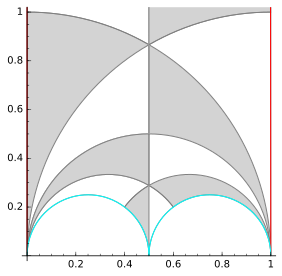
\includegraphics[width=0.4\textwidth]{X0-4.png}
	\caption{$\Gamma_0(4)$ 或 $\Gamma_1(4)$ 的一个基本区域, 以 SageMath 软件绘制.}
\end{figure}

\section{偶数权维数公式}\label{sec:dimension-formula-even}
本节将应用 Riemann--Roch 定理 \ref{prop:RR} 来计算模形式空间的维数. 我们关注的是权为 $2k$ 的模形式, 其中 $k \in \Z$. 条件 $f \modact{2k} \gamma = f$ 等价于说线丛 $f (\dd \tau)^{\otimes k} \in \Gamma(\mathcal{H}, \Omega_{\mathcal{H}}^{\otimes k})$ 对 $\gamma$ 不变; 见 \eqref{eqn:even-weight-equivalence}. 定义
\[ \mathcal{H}' := \mathcal{H} \smallsetminus \{ \Gamma\; \text{的椭圆点} \}, \quad Y(\Gamma)' := \Gamma\backslash\mathcal{H}' . \]
那么 $\Gamma$ 在 $\mathcal{H}'$ 上的作用自由, 商映射 $p: \mathcal{H}^* \to X(\Gamma)$ 限制为 $\mathcal{H}' \to Y(\Gamma)'$, 这成为一个 $\overline{\Gamma}$-主丛, 特别地, 它也是复叠映射.

透过拉回, $\overline{\Gamma}$ 自然地作用于 $\mathcal{H}$ 上的微分形式 (回忆引理 \ref{prop:fractional-transform-d}), 继而在其 $k$-次张量幂上也有诱导作用. 于是
\begin{equation}\label{eqn:modular-form-as-section-0}\begin{tikzcd}[column sep=tiny]
	\omega \arrow[phantom, r, "\in" description] \arrow[mapsto, d] & \Gamma\left(Y(\Gamma)', \Omega_{Y(\Gamma)'}^{\otimes k}\right) \arrow[d, "\simeq"']  \\
	p^*\omega = f (\dd\tau)^{\otimes k} \arrow[phantom, r, "\in" description] & \Gamma\left( \mathcal{H}', \Omega_{\mathcal{H}'}^{\otimes k} \right)^{\Gamma-\text{不变}} \\
	f \arrow[mapsto, u] \arrow[phantom, r, "\in"] & \left\{ f: \mathcal{H}' \to \CC \;\text{全纯},\; \forall \gamma \in \Gamma,\; f\modact{2k} \gamma = f \right\} \arrow[u, "\simeq", "\text{据 \eqref{eqn:even-weight-equivalence}}"']
\end{tikzcd}\end{equation}
我们来解释第一个同构: 既然 $\mathcal{H}'$ 不含椭圆点, 引理 \ref{prop:nbhd-elliptic} 说明任意 $\eta \in \mathcal{H}'$ 总有开邻域 $U$ 使得 $\left\{ \gamma U : \gamma \in \Gamma \right\}$ 不交, 对开集 $V := p(U)$ 自然就有
\[ \Gamma\left( V, \Omega_{Y(\Gamma)'}^{\otimes k}\right) \simeq \Gamma\left( U, \Omega_U^{\otimes k} \right) = \Gamma\left(p^{-1}(V), \Omega_{\mathcal{H}'}^{\otimes k} \right)^{\Gamma-\text{不变}}. \]
这些同构也能在 $Y(\Gamma)'$ 的开集及其原像上局部地考量. 为了将模形式刻画为线丛的截面, 我们必须进一步考虑椭圆点和尖点附近的性状, 并和 $X(\Gamma)$ 的复结构相比较.

\begin{asparaenum}[(A)]
	\item 令 $\eta \in \mathcal{H}$. 记 $y := p(\eta) \in Y(\Gamma)$. 取引理 \ref{prop:glueing-holomorphy} 提供的开邻域 $V \ni \eta$, 满足 $V = p(U)$, 其中 $U$ 是 $\tau \in \mathcal{H}$ 的 $\overline{\Gamma}_\tau$-不变开邻域, 其中或者无椭圆点, 或以 $\eta$ 为唯一椭圆点. 我们有交换图表
	\[\begin{tikzcd}
		\eta \arrow[phantom, d, "\in" description, sloped] \arrow[mapsto, r] & 0 \arrow[phantom, d, "\in" description, sloped] \\
		U \arrow[r, "\sim"] \arrow[twoheadrightarrow, d, "p"' inner sep=1em] & \mathcal{D} \arrow[twoheadrightarrow, d, "{f_e: z \mapsto z^e}" inner sep=1em] \\
		V \arrow[r, "\sim"] & \mathcal{D}
	\end{tikzcd} \qquad e := e(y), \]
	其中水平箭头都是全纯同构, 而 $\overline{\Gamma}_\tau$ 在 $U$ 上的作用对用到 $\mu_e$ 在 $\mathcal{D} = \{z \in \CC: |z| < 1 \}$ 上的乘法作用. 特别地, $p$ 限制在 $U \smallsetminus \{\eta\}$ 上是 $V \smallsetminus \{y\}$ 的 $e$ 次复叠映射.
	
	设模形式 $f$ 限制在 $U \smallsetminus \{\eta\}$ 上对应于 $\omega \in \Gamma\left(V \smallsetminus \{y\}, \Omega_{Y(\Gamma)'}^{\otimes k}\right)$, 或用上图赋予 $U$, $V$ 的局部坐标 (统称为 $z$) 写作
	\begin{gather*}
		\omega = g(z) (\dd z)^{\otimes k}, \qquad g: \mathcal{D} \smallsetminus \{0\} \xrightarrow{\text{全纯}} \CC , \\
		p^* \omega = g(z^e) (\dd z^e)^{\otimes k} = e^k z^{k(e-1)} g(z^e) (\dd z)^{\otimes k}.
	\end{gather*}
	为了使 $f$ 或 $p^* \omega$ 在 $U$ 上全纯, 条件遂变为 $g$ 在 $z=0$ 处亚纯, 而且
	\begin{gather}\label{eqn:modular-form-as-section-1}
		k(e-1) + e \cdot \ord_\eta(\omega) = k(e-1) + e \cdot \ord_{0}(g) = \ord_\eta(f)
	\end{gather}
	非负.

%	\item 若 $\eta \in \mathcal{H}$ 不是椭圆点, 上述讨论中 $e = 1$, 而 \eqref{eqn:modular-form-as-section-1} 非负的条件化作 $\ord_\eta(\omega) \geq 0$, 亦即 $\omega$ 在 $\eta$ 附近全纯.
	\item 接着考虑任意 $t \in \mathcal{C}_\Gamma$ 附近的情形, 对应的尖点是 $c := p(t)$. 不失一般性且设 $t = \infty$. 对之可取充分小的开邻域 $H^\circ = \{ \tau: \Im(\tau) > a \}$ (其中 $a \in \R_{>0}$) 以及 $X(\Gamma)$ 在 $c$ 附近的局部坐标 $q: \Gamma_t \backslash H^\circ \sqcup \{\infty\} \to \CC$, 形如
	\[ q: \tau \mapsto \exp(2\pi i\tau/h) \]
	其中的常数 $h \in \R_{>0}$ 只和尖点 $c$ 与 $\Gamma$ 相关; 见 \eqref{eqn:cusp-width}. 和前一情形类似, 将对应于 $f|_{H^\circ}$ 的 $\omega$ 在局部坐标 $q$ 下写作 $g(q) (\dd q)^{\otimes k}$, 那么
	\[ p^*\omega = g\left( q(\tau) \right) \cdot \left(\dfrac{2\pi i}{h}\right)^k q(\tau)^k (\dd\tau)^{\otimes k} . \]
	为了使 $f$ 在 $t$ 处全纯, 其条件为 $g(q) q^k$ 在 $q=0$ 附近有界, 等价的说法是下式非负.
	\begin{gather}\label{eqn:modular-form-as-section-2}
		k + \ord_c(\omega) = k + \ord_{q=0}(g) = \ord_t(f).
	\end{gather}

	此外, $f$ 在 $t$ 处消没当且仅当 $\lim_{q \to 0} g(q)q^k = 0$, 亦即 \eqref{eqn:modular-form-as-section-2} 为正. 回忆到 $f$ 在尖点处的消没次数由它对 $q$ 的 Fourier 展开定义.
\end{asparaenum}

\begin{theorem}\label{prop:dimension-formula}
	我们有自然同构
	\[\begin{tikzcd}
		M_{2k}(\Gamma) \arrow[r, "\sim"] & \Gamma\left( X(\Gamma), \; \Omega_{X(\Gamma)}^{\otimes k} (\lfloor k D_\Gamma \rfloor) \right) \\
		S_{2k}(\Gamma) \arrow[r, "\sim"] \arrow[phantom, u, "\subset" sloped] & \Gamma\left( X(\Gamma), \; \Omega_{X(\Gamma)}^{\otimes k}(\lfloor k D_\Gamma \rfloor - \sum_{c: \text{尖点}} c) \right)  \arrow[phantom, u, "\subset" sloped];
	\end{tikzcd}\]
	特别地, 取 $k=1$ 给出 $S_2(\Gamma) \rightiso \Gamma\left( X(\Gamma), \Omega_{X(\Gamma)} \right)$.
\end{theorem}
\begin{proof}
	鉴于 $D_\Gamma$ 的定义 \ref{def:Hodge-class}, 这是之前关于 \eqref{eqn:modular-form-as-section-0}, \eqref{eqn:modular-form-as-section-1} 和 \eqref{eqn:modular-form-as-section-2} 的讨论的直接结论.
\end{proof}

\begin{corollary}\label{prop:M-finiteness}
	空间 $M_{2k}(\Gamma)$ 总是有限维的.
\end{corollary}
\begin{proof}
	这是定理 \ref{prop:RR} 的一部分.
\end{proof}

\begin{theorem}\label{prop:dimension-formula-explicit}
	以 $\epsilon_\infty$ 表 $X(\Gamma)$ 的尖点个数, $g$ 表 $X(\Gamma)$ 的亏格, $L_\Gamma$ 如定义 \ref{def:Hodge-class}, 则
	\begin{align*}
		\dim_{\CC} M_{2k}(\Gamma) & = \begin{cases}
		0, & k < 0, \\
		1, & k=0, \\
		g, & k=1 \wedge \epsilon_\infty=0, \\
		g + \epsilon_\infty - 1, & k=1 \wedge \epsilon_\infty > 0, \\
		\dim_{\CC} S_{2k}(\Gamma) + \epsilon_\infty, & k > 1;
	\end{cases} \\
	\dim_{\CC} S_{2k}(\Gamma) & = \begin{cases}
		0, & k < 0, \\
		0, & k=0 \wedge \epsilon_\infty > 0, \\
		1, & k=0 \wedge \epsilon_\infty = 0, \\
		g, & k=1, \\
		\deg\left( k K_{X(\Gamma)} + \lfloor k D_\Gamma \rfloor \right) - g + 1 - \epsilon_\infty, & k > 1.
	\end{cases}\end{align*}
	此外, 当 $k > 1$ 时
	\[ \dim_{\CC} S_{2k}(\Gamma) \geq (k-1) \deg(L_\Gamma) + g - 1. \]
\end{theorem}

因为定理 \ref{prop:D-estimate} 蕴涵 $\deg(L_\Gamma) > 0$, 上述估计说明当 $k \gg 0$ 时, 权为 $2k$ 的模形式是十分丰富的; 关于 $M_{2k}(\Gamma)$ 的全套理论并不是空中楼阁.

\begin{proof}
	基本工具是 Riemann--Roch 定理. 引入方便的符号
	\[ \left\lfloor kL_\Gamma \right\rfloor := k K_{X(\Gamma)} + \lfloor k D_\Gamma \rfloor \; \in \Pic(X(\Gamma)); \]
	命题 \ref{prop:C-section-L} 和定理 \ref{prop:dimension-formula} 一同给出
	\begin{align*}
		\dim_{\CC} M_{2k}(\Gamma) & = \ell\left( k K_{X(\Gamma)} + \lfloor kD_\Gamma \rfloor \right) = \ell\left( \lfloor k L_\Gamma \rfloor \right), \\
		\dim_{\CC} S_{2k}(\Gamma) & = \ell\left( \lfloor k L_\Gamma \rfloor - \sum_{c: \text{尖点}} c \right).
	\end{align*}
	当 $k=0$ 时我们得到 $\ell(0)=1$, 相应的模形式都是常值函数; 非零常值函数是尖点形式当且仅当 $\epsilon_\infty=0$. 这和断言一致.
	
	当 $k \geq 1$ 时, 命题 \ref{prop:floor-Hodge} 给出
	\begin{equation}\label{eqn:dimension-formula-deg-bound}
		\deg\left( \lfloor k L_\Gamma \rfloor \right) \geq 2g - 2 + \epsilon_\infty + (k-1) \deg(L_\Gamma),
	\end{equation}
	从而
	\begin{equation}\label{eqn:dimension-formula-deg-bound-cusp}
	\begin{aligned}
		\deg\left( \lfloor k L_\Gamma \rfloor - \sum_{c: \text{尖点}} c \right) & = \deg\left( \lfloor k L_\Gamma \rfloor \right) - \epsilon_\infty \\
		& \geq 2g - 2 + (k-1)\deg(L_\Gamma).
	\end{aligned}\end{equation}
	定理 \ref{prop:D-estimate} 断言 $\deg(L_\Gamma) > 0$, 因而当 $k > 1$ 时 \eqref{eqn:dimension-formula-deg-bound} 和 \eqref{eqn:dimension-formula-deg-bound-cusp} 都 $> 2g-2$. 于是可以运用 Riemann--Roch 定理 \ref{prop:RR} 及其后的注记 \ref{rem:RR} 来对 $k > 1$ 计算
	\begin{align*}
		\ell\left( \lfloor k L_\Gamma \rfloor \right) & = \deg\left( \lfloor k L_\Gamma \rfloor\right) - g + 1 \\
		& = k(2g-2) + \deg\lfloor k D_\Gamma \rfloor - g + 1, \\
		\ell\left( \lfloor k L_\Gamma \rfloor - \sum_{c: \text{尖点}} c \right) & = \deg\left( \lfloor k L_\Gamma \rfloor\right) - g + 1 - \epsilon_\infty \\
		& \geq g - 1 + (k-1) \deg(L_\Gamma) \quad (\because\; \text{命题 \ref{prop:floor-Hodge}}).
	\end{align*}
	两则等式分别给出 $M_{2k}(\Gamma)$ 和 $S_{2k}(\Gamma)$ 在 $k > 1$ 时的维数公式, 不等式给出断言中维数的下界.
	
	当 $k < 0$ 时, 命题 \ref{prop:floor-Hodge} 另一边的简单估计给出
	\[ \deg\left( \lfloor k L_\Gamma \rfloor \right) \leq k \deg(L_\Gamma) < 0. \]
	于是引理 \ref{prop:low-degree-vanishing} 给出 $\dim M_{2k}(\Gamma) = \ell\left( \lfloor k L_\Gamma \rfloor \right) = 0$, 从而也有 $S_{2k}(\Gamma) = \{0\}$.
	
	剩下 $k=1$ 情形. 考虑除子类 $\lfloor L_\Gamma \rfloor = K_{X(\Gamma)} + \sum_{c: \text{尖点}} c$. 根据注记 \ref{rem:RR}, 此时总有
	\[ \dim_{\CC} S_2(\Gamma) = \ell(K_{X(\Gamma)}) = g. \]
	若进一步设 $\epsilon_\infty = 0$, 则 $\dim_{\CC} M_2(\Gamma) = \dim_{\CC} S_2(\Gamma) = g$. 若 $\epsilon_\infty > 0$, 则
	\[ \deg\left( \lfloor L_\Gamma \rfloor \right) = 2g-2 + \epsilon_\infty > 2g-2, \]
	于是 $\dim_{\CC} M_2(\Gamma) = \ell\left( K_{X(\Gamma)} + \sum_{c: \text{尖点}} c \right) = g + \epsilon_\infty - 1$. 证毕.
\end{proof}

\begin{example}\label{eg:dimension-Gamma04}
	代入例 \ref{eg:Gamma04-genus} 计算过的 $\Gamma_0(4)$ 作为演示. 此时无椭圆点,
	\[ \epsilon_\infty = 3, \quad g = 0, \quad \deg kK_{X(\Gamma_0(4))} = -2k, \quad \deg \lfloor k D_{\Gamma_0(4)} \rfloor = 3k; \]
	参看注记 \ref{rem:RR}. 由此导出
	\begin{equation*}\begin{aligned}
		\dim_{\CC} S_{2k}(\Gamma_0(4)) & = \begin{cases}
			0, & k = 0, 1 \\
			k - 2, & k \geq 2,
		\end{cases} \\
		\dim_{\CC} M_{2k}(\Gamma_0(4)) & = k + 1, \quad k \geq 0.
	\end{aligned}\end{equation*}
	对于 $\Gamma_1(4)$, 偶数权的维数公式丝毫不差; 见例 \ref{eg:Gamma14-genus} 的讨论.
\end{example}

最后, 我们从线丛的角度描述模形式的零点.
\begin{proposition}\label{prop:modular-form-zeros}
	设 $f \in M_{2k}(\Gamma) \smallsetminus \{0\}$, 则
	\[ \sum_{x \in Y(\Gamma)} \dfrac{\ord_\tau(f)}{e(x)} + \sum_{x \in X(\Gamma) \smallsetminus Y(\Gamma)} \ord_\tau(f) = k \deg(L_\Gamma), \]
	其中 $\tau$ 是 $x$ 在 $\mathcal{H}^*$ 中的任意代表元, $f$ 在尖点处的消没次数以 Fourier 展开来定义.
\end{proposition}
\begin{proof}
	从早先的论证可知 $f$ 对应到 $\Omega_{X(\Gamma)}^{\otimes k}$ 的亚纯截面 $\omega$, 不恒为零. 按附录 \ref{sec:RR} 的符号体系,
	\[ \sum_{x \in X(\Gamma)} \ord_x(\omega) = \deg \left(\divisor\left( \Omega_{X(\Gamma)}^{\otimes k}, \omega \right)\right) = k \deg K_{X(\Gamma)} = k(2g-2). \]

	在 \eqref{eqn:modular-form-as-section-1} 已观察到当 $x \in Y(\Gamma)$, 而 $\tau \in \mathcal{H}$ 为其原像时 $\ord_\tau(f) = k(e(x)-1) + e(x) \ord_x(\omega)$. 对于尖点 $x \in X(\Gamma) \smallsetminus Y(\Gamma)$ 及其原像 $t \in \mathcal{H}^*$, \eqref{eqn:modular-form-as-section-2} 表明 $\ord_t(f) = k + \ord_x(\omega)$. 加总得到
	\[ \sum_{x \in Y(\Gamma)} \left( \dfrac{\ord_\tau(f)}{e(x)} - k\left( 1 - \dfrac{1}{e(x)} \right)\right) + \sum_{x \in X(\Gamma) \smallsetminus Y(\Gamma)} \ord_t(f) - k \epsilon_\infty = k(2g - 2). \]
	再以定理 \ref{prop:D-estimate} 或 $L_\Gamma$ 的定义整理出 $\deg(L_\Gamma)$ 便是.
\end{proof}

命题 \ref{prop:modular-form-zeros} 也适用于亚纯模形式 (回顾定义 \ref{def:modular-form-gen}), 论证完全相同.

\section{应用举隅}\label{sec:dimension-full}
对任意 $N \in \Z_{\geq 1}$ 和 $k \in \Z$ 定义 $M_k(N) := M_k(\Gamma(N))$, $S_k(N) := S_k(\Gamma(N))$. 置 $X(N) := X(\Gamma(N))$.

当 $N=1$ 时, 我们于 \S\ref{sec:Eisenstein-fulllevel} 业已造出相应的 Eisenstein 级数 $E_k \in M_k(1)$ (要求 $k \in 2\Z_{\geq 2}$), 并于 \S\ref{sec:j-invariant} 定义了模判别式 $\Delta \in S_{12}(1)$. 模曲线 $X(1)$ 的信息十分明白:
\[ g = 0, \quad 2g - 2 = -2, \quad \text{尖点代表元}: \infty; \]
椭圆点代表元是 $i$ 和 $\rho = e^{2\pi i/6}$, 约定 \ref{conv:e} 定义的 $e(\cdot)$ 为
\[ e(i) = 2, \quad e(\rho) = 3. \]
这不外是命题 \ref{prop:elliptic-pt-cyclic} 的内容. 因此
\[ \deg(L_\Gamma) = -2 + 1 + \frac{1}{2} + \frac{2}{3} = \frac{1}{6}; \]
当然, 这也可以从 $\mes(Y(1)) = \frac{\pi}{3}$ 来计算 (命题 \ref{prop:hyperbolic-volume}). 本节第一个应用是确定 $E_4, E_6$ 的零点.

\begin{proposition}\label{prop:zeros-E4-E6}
	我们有 $E_4(\rho) = E_6(i) = 0$, 而且它们分别是 $E_4, E_6$ 的唯一零点, 同为一阶.
\end{proposition}
\begin{proof}
	从 $Y(1)$ 扣掉椭圆点得到 $Y(1)'$. 因为 $E_4, E_6$ 在 $\infty$ 处全纯非零, 代入命题 \ref{prop:modular-form-zeros} 得到
	\begin{align*}
		\frac{\ord_i(E_4)}{2} + \frac{\ord_\rho(E_4)}{3} + \sum_{x \in Y(1)'} \ord_\tau(E_4) & =  \frac{1}{3}, \\
		\frac{\ord_i(E_6)}{2} + \frac{\ord_\rho(E_6)}{3} + \sum_{x \in Y(1)'} \ord_\tau(E_6) & =  \frac{1}{2}.
	\end{align*}
	因此 $E_4$ (或 $E_6$) 唯一的零点在 $\rho$ (或 $i$) 处, 同为一阶.
\end{proof}

\begin{theorem}\label{prop:dimension-full}
	对于任意 $k \in 2\Z$, 当 $k < 0$ 或  $k = 2$ 时 $M_k(1) = \{0\}$; 当 $k \geq 4$ 时我们有
	\begin{gather*}
		M_k(1) = S_k(1) \oplus \CC E_k, \\
		\dim_{\CC} S_k(1) = \begin{cases}
			\lfloor \frac{k}{12} \rfloor - 1, & k \equiv 2 \pmod {12}, \\
			\lfloor \frac{k}{12} \rfloor, & k \not\equiv 2 \pmod {12};
		\end{cases}
	\end{gather*}
	特别地, $S_k(1)$ 非零当且仅当 $k \geq 12$ 而 $k \neq 14$.
\end{theorem}
\begin{proof}
	在定理 \ref{prop:dimension-formula-explicit} 中代入 $g=0$ 和 $\epsilon_\infty=1$, 得出 $M_2(1) = \{0\}$. 故以下着力探讨 $M_k(1)$, 其中 $k \in 2\Z_{\geq 2}$.
	
	设 $f \in M_k(1)$. 已知 $E_k(\tau)$ 在 $\infty$ 的 Fourier 展开常数项为 $1$, 故 $f$ 有唯一表法
	\[ f = g + c E_k, \quad g \in S_k(1), \; c \in \CC; \]
	事实上 $c$ 无非是 $f$ 的常数项. 这就说明了 $M_k(1) = S_k(1) \oplus \CC E_k$. 下面用定理 \ref{prop:dimension-formula-explicit} 计算 $\dim_{\CC} S_k(1)$. 此时
	\begin{gather*}
		D_{\Gamma(1)} = \frac{1}{2} \cdot i + \frac{2}{3} \cdot \rho + \infty, \\
		\deg \left\lfloor \frac{k}{2} D_{\Gamma(1)} \right\rfloor = \deg\left( \left\lfloor\frac{k}{4}\right\rfloor \cdot i + \left\lfloor\frac{k}{3}\right\rfloor \cdot \rho + \frac{k}{2} \cdot \infty \right) = \left\lfloor\frac{k}{4}\right\rfloor + \left\lfloor\frac{k}{3}\right\rfloor + \frac{k}{2}, \\
		\frac{k}{2} \deg K_{X(1)} = -k.
	\end{gather*}
	故 $\dim_{\CC} S_k(1) = \lfloor\frac{k}{4}\rfloor + \lfloor\frac{k}{3}\rfloor - \frac{k}{2}$. 为了确定取整运算的值, 表 $k$ 为 $2(6q + r)$, 其中 $0 \leq r < 6$,
	\[\begin{array}{c|c|c|c|c}
		r & \lfloor \frac{k}{4} \rfloor & \lfloor \frac{k}{3} \rfloor & \frac{k}{2} & \lfloor\frac{k}{4}\rfloor + \lfloor\frac{k}{3}\rfloor - \frac{k}{2} \\ \hline
		0 & 3q & 4q & 6q & q \\
		1 & 3q & 4q & 6q+1 & q-1 \\
		2 & 3q+1 & 4q+1 & 6q+2 & q \\
		3 & 3q+1 & 4q+2 & 6q+3 & q \\
		4 & 3q+2 & 4q+2 & 6q+4 & q \\
		5 & 3q+2 & 4q+3 & 6q+5& q \\
	\end{array}\]
	因为 $\lfloor \frac{k}{12} \rfloor = q$, 这就验证了 $\dim_{\CC} S_k(1)$ 的公式.
\end{proof}

回忆 \S\ref{sec:Eisenstein-fulllevel} 构造的 Eisenstein 级数 $E_k$, $G_k$ 以及定义 \ref{def:Delta} 中的模判别式
\[ \Delta = q \prod_{n=1}^\infty (1-q^n)^{24} = \sum_{n \geq 1} \tau(n) q^n \; \in S_{12}(1), \quad q = e^{2\pi i\tau}. \]
注意到 $\tau(1) = 1$. 以下论证将涉及定义 \ref{def:sigma-function} 的除数函数 $\sigma_r$, 其中 $r \geq 0$.

\begin{lemma}\label{prop:E4-E6}
	存在整数列 $a_2, a_3, \ldots$ 和 $b_2, b_3, \ldots$ 使得
	\begin{align*}
		E_4(\tau)^3 & = 1 + 720\left( q + \sum_{n \geq 2} a_n q^n \right), \\
		E_6(\tau)^2 & = 1 - 1008\left( q + \sum_{n \geq 2} b_n q^n \right).
	\end{align*}
\end{lemma}
\begin{proof}
	应用 $E_k$ 的 Fourier 展开 \eqref{eqn:E-formula}	配合 \eqref{eqn:Bernoulli-table} 的资料 $B_4 = -\frac{1}{30}$ 和 $B_6 = \frac{1}{42}$ 来计算
	\begin{equation*}\begin{aligned}
		E_4(\tau) & = 1 + \dfrac{2 \cdot 4}{-B_4} \sum_{n \geq 1} \sigma_3(n) q^n \\
		& = 1 + 240 \left( q + \sum_{n \geq 2} \sigma_3(n) q^n \right) \\
		E_6(\tau) & = 1 + \dfrac{2 \cdot 6}{-B_6} \sum_{n \geq 1} \sigma_5(n) q^n \\
		& = 1 - 504 \left( q + \sum_{n \geq 2} \sigma_5(n) q^n \right).
	\end{aligned}\end{equation*}
	它们可视同以 $q$ 为变元的整系数形式幂级数环 $\Z\llbracket q \rrbracket$ 的元素. 二项式定理遂给出
	\begin{align*}
		E_4^3 & \in \left( 1 + 240 q (1+q\Z\llbracket q \rrbracket) \right)^3 \subset 1 + 720 q + 720 q^2 \Z\llbracket q \rrbracket, \\
		E_6^2 & \in \left( 1 - 504 q (1+q\Z\llbracket q \rrbracket) \right)^2 \subset 1 - 1008 q + 1008 q^2 \Z\llbracket q \rrbracket.
	\end{align*}
	明所欲证.
\end{proof}

\begin{corollary}\label{prop:Delta-Eisenstein}
	空间 $S_{12}(1)$ 由 $\Delta$ 张成, 并且
	\[ \Delta = \frac{1}{1728} \left( E_4^3 - E_6^2 \right). \]
\end{corollary}
\begin{proof}
	定理 \ref{prop:dimension-full} 蕴涵 $\dim_{\CC} S_{12}(1) = 1$, 因而 $S_{12}(1) = \CC\Delta$. 引理 \ref{prop:E4-E6} 指出 $E_4^3 - E_6^2 = 1728 q + \cdots \in S_{12}(1)$ (省略号代表 $q$ 的高次项), 它必为 $\Delta$ 的倍数. 另一方面, $\Delta = q + \cdots$, 综之有 $\Delta = \frac{1}{1728} \left( E_4^3 - E_6^2 \right)$.
\end{proof}

今将以 $E_4$ 和 $E_6$ 来生成级为 $\Gamma(1)$ 的所有模形式. 以下定义 $\CC$-代数 $M(1) := \bigoplus_{k \in \Z} M_k(1)$ 及其理想 $S(1) := \bigoplus_{k \in \Z} S_k(1)$. 顺带一提, 它们还具有源自权 $k$ 的分次的结构, 一般理论详见 \cite[\S 7.4]{Li1}.

\begin{lemma}\label{prop:E4-E6-indep}
	定义 $M(1)$ 如上, 则 $E_4, E_6 \in M(1)$ 在 $\CC$ 上代数无关 (见 \cite[\S 8.8]{Li1}): 换言之, 任意多项式 $f \in \CC[X,Y]$ 若满足 $f(E_4, E_6) = 0 \in M(1)$, 则 $f$ 是零多项式.
\end{lemma}
\begin{proof}
	设 $f = \sum_{a,b} c_{ab} X^a Y^b \in \CC[X,Y]$ 满足 $f(E_4, E_6)=0$. 按定义, 来自不同权的部分在 $M(1)$ 中线性无关, 故对所有 $k \geq 0$, 多项式 $f_k := \sum_{4a+6b=k} c_{ab} X^a Y^b$ 都满足 $f_k(E_4, E_6) = 0$.
	
	今假设 $E_4, E_6$ 在 $\CC$ 上代数相关, 并取极小的正整数 $k$ 使得存在非零之 $f = \sum_{4a+6b=k} c_{ab} X^a Y^b$ 满足 $f(E_4, E_6) = 0$. 代入 $\tau = \rho$, 因为 $E_4(\rho)=0$ 而 $E_6(\rho) \neq 0$, 从 $f$ 的形式可知 $X \mid f$; 同理, 代入 $\tau = i$ 可知 $Y \mid f$, 于是考虑 $g := f/XY$ 可得 $g(E_4, E_6)=0$, 其中 $g = \sum_{4a+6b=k-10} c_{a+1, b+1} X^a Y^b$, 这同 $k$ 极小相矛盾.
\end{proof}

\begin{theorem}
	定义 $M(1)$, $S(1)$ 如上, 则
	\begin{align*}
		M(1) & = \CC[E_4, E_6], \\
		S(1) & = \Delta \cdot M(1).
	\end{align*}
	事实上, 我们有 $\CC$-代数的同构 $\varphi: \CC[X,Y] \rightiso M(1)$, 映 $f(X,Y)$ 为 $f(E_4, E_6)$.
\end{theorem}
\begin{proof}
	命题 \ref{prop:k-parity} 表明 $M_{\text{奇数}}(1) = \{0\}$. 定理 \ref{prop:dimension-full} 则表明 $M_{\text{负偶数}}(1) = \{0\} = M_2(1)$. 因此只需考虑权 $k \in 2\Z$, $k \geq 2$ 的情形; 留意到 $M_0(1) = \CC$ (常值函数).

	首先说明 $f \mapsto f\Delta$ 给出同构 $M_k(1) \rightiso S_{k+12}(1)$. 单性自明, 今假设 $g \in S_{k+12}(1)$. 根据 $\Delta$ 的无穷乘积展开知 $\Delta$ 在 $\infty$ 有一阶零点, 在 $\mathcal{H}$ 上无零点, 由之易见 $g/\Delta \in M_k(1)$, 从而得到满性. 然而定理 \ref{prop:dimension-full} 蕴涵 $w < 12 \implies S_w(1) = \{0\}$, 故 $S(1) = \Delta M(1)$.

	以下证明 $\left\{ E_4^a E_6^b : a,b \in \Z_{\geq 0},\; 4a+6b=k \right\}$ 生成向量空间 $M_k(1)$. 已知 $M_2(1) = \{0\}$, 而 $M_4(1)$ 和 $M_6(1)$ 皆 $1$ 维, 故仅须处理 $k > 6$ 情形. 因为 $k$ 是正偶数, 根据初等数论可知存在 $a,b \in \Z_{\geq 0}$ 使得 $\frac{k}{2} = 2a+3b$. 若 $f \in M_k(1)$ 在 $\infty$ 处的常数项是 $c$, 则 $f_1 := f - c E_4^a E_6^b \in S_k(1)$. 若 $f_1=0$ 则停止, 否则存在 $g \in M_{k-12}(1)$ 满足 $f_1 = \Delta \cdot g$. 然而 $\Delta = \frac{1}{1728} (E_4^3 - E_6^2)$; 对 $g$ 递归即可.
	
	于是断言中的 $\CC$-代数同态 $\varphi: \CC[X,Y] \to M(1)$ 是满的, 其单性则是引理 \ref{prop:E4-E6-indep} 的内容. 
\end{proof}

\begin{exercise}\label{exo:M(1)-integral}
	证明 $M(1)$ 具有一个分次子环 $M(1)_{\Z}$, 使得
	\begin{compactitem}
		\item 它是分次的, 亦即作为 $\Z$-模有直和分解 $M(1)_{\Z} = \bigoplus_k \left( M_k(1) \cap M(1)_{\Z} \right)$;
		\item $M(1)$ 作为 $\CC$-向量空间由 $M(1)_{\Z}$ 生成;
		\item 所有属于 $M(1)_{\Z}$ 的模形式其 Fourier 系数都是整数.
	\end{compactitem}
	我们称这给出 $M(1)$ 的一个整结构. 进一步描述 $M(1)_{\Z}$ 的分次理想 $M(1)_{\Z} \cap S(1)$.
	
	\begin{hint}
		取 $M(1)_{\Z}$ 为所有 Fourier 系数均为整数的模形式给出的子环, 并应用前述定理\footnote{相关的整性问题可以参考 Serge Lang 的 \textit{Introduction to Modular Forms} (Grundlehren der mathematischen Wissenschaften, Volume 222), Chapter X, Theorems 4.2---4.4. 论证是初等的.}. 对一般同余子群也有类似的整结构, 但需要更强有力的几何工具, 见 \S\ref{sec:geometric-modular-form}.
	\end{hint}
\end{exercise}

\begin{example}[Ramanujan 同余] \index{Ramanujan $\tau$ 函数} \index{Ramanujan 同余 (Ramanujan's congruences)}
	以下是维数公式一个有趣而且影响深远的应用. 回忆 $\Delta = \sum_{n \geq 1} \tau(n) q^n$, 并注意到 $691$ 是素数. 兹断言当 $n \in \Z_{\geq 1}$ 时,
	\[ \tau(n) \equiv \sigma_{11}(n) \pmod {691}. \]
	根据约定 \ref{conv:new-G}, 我们有
	\[ \mathcal{G}_{12}(\tau) := \dfrac{-B_{12}}{24} + \sum_{n \geq 1} \sigma_{11}(n) q^n \; \in M_{12}(1). \]
	另一方面, 考虑 $M_{12}(1)$ 的元素
	\[ \dfrac{E_4^3}{720} + \dfrac{E_6^2}{1008} \;\in \frac{1}{420} + q^2 \Z\llbracket q\rrbracket; \]
	此处用上了引理 \ref{prop:E4-E6} 及其证明中的记号, 以及 $1728 \times 420 = 720 \times 1008$. 因为 $S_{12}(1) = \CC\Delta$ 而 $\dim_{\CC} M_{12}(1) = 2$, 由此得知 $M_{12}(1)$ 的元素都唯一表作 $a \Delta + b\left(\dfrac{E_4^3}{720} + \dfrac{E_6^2}{1008}\right)$ 之形.
	
	接着以此表达 $\mathcal{G}_{12}$. 我们比较 $q^0$ 和 $q^1$ 的系数来确定 $a,b$: 查阅 \eqref{eqn:Bernoulli-table} 知 $B_{12} = \frac{-691}{2730}$, 故 $\mathcal{G}_{12}$ 的常数项可以直接计算为
	\[ \dfrac{-B_{12}}{24} = \dfrac{691}{156} \cdot \dfrac{1}{420}. \]
	此外 $q^1$ 在 $\mathcal{G}_{12}$ 中和在 $\Delta$ 中的系数同为 $1$. 综之, $\mathcal{G}_{12} = \Delta + \dfrac{691}{156} \cdot \left(\dfrac{E_4^3}{720} + \dfrac{E_6^2}{1008}\right)$.
	
	接着比较上式两边 $q^n$ 的系数 ($n=1,2,\ldots$). 首先 $\mathcal{G}_{12}$ 的系数为 $\sigma_{11}(n) \in \Z$, 而 $\Delta$ 的系数 $\tau(n)$ 也是整数; 因为 $\dfrac{E_4^3}{720} + \dfrac{E_6^2}{1008}$ 的 $q^n$ 系数亦是整数, 相减可得
	\[ \tau(n) - \sigma_{11}(n) \; \in \Z \cap \left(\dfrac{691}{156} \cdot \Z\right) \subset 691\Z. \]
	此即所求之 Ramanujan 同余.
	
	同余关系可以进一步涵摄 $n=0$ 情形. 合理地定义 $\tau(0)=0$. 虽然 $\mathcal{G}_{12}$ 的常数项 $\dfrac{-B_{12}}{24}$ 非整, 但它属于 $\Q$ 的子环 $\Z_{(691)} := \left\{ \frac{v}{u} : u,v \in \Z, \; \text{gcd}(u, 691)=1 \right\}$ (这是环 $\Z$ 对理想 $691 \Z$ 的局部化, 见 \cite[\S 5.3]{Li1}), 其中 $691$ 依然生成极大理想. 置 Fourier 系数于环 $\Z_{(691)}$, 则有 $\frac{-B_{12}}{12} \equiv 0 = \tau(0) \pmod{ 691\Z_{(691)}}$. 当 $n \geq 1$ 时, 在 $\Z_{(691)}$ 中考量 Ramanujan 同余也不损失任何信息.
\end{example}

上述论证可能给人一种印象, 仿佛 Ramanujan 同余仅只是一个精致的数值巧合. 其实尖点形式和 Eisenstein 级数之间的同余是数论中的一类广泛现象, 根源在几何, \emph{$p$-进模形式}理论是理解它的一把钥匙. 为此, 精细爬梳模空间的算术/几何性质当然是必不可少的.

\begin{exercise}\label{exo:Deligne-congruence}
	设 $p \geq 3$ 为素数. 证明 Eisenstein 级数 $E_{p-1}$ 的所有 Fourier 系数都属于 $\Z_{(p)}$ (定义同上), 而且除了常数项 $1$, 其余 Fourier 系数都属于理想 $p \Z_{(p)}$.

	\begin{hint}
		运用关于 Bernoulli 数的 von Staudt--Clausen 定理来研究 $B_{p-1}$ 的分子与分母, 然后代入 \eqref{eqn:E-formula}.
	\end{hint}
\end{exercise}

\section{亚纯模形式的存在性}
选定余有限 Fuchs 群 $\Gamma \subset \SL(2,\R)$. 本节的结论仅在定理 \ref{prop:dimension-formula-odd} 用到. 所有 Riemann 曲面均默认为紧的.

\begin{theorem}
	设 $k \in \Z$. 存在权为 $2k$, 级为 $\Gamma$ 而且不恒为零的亚纯模形式.
\end{theorem}
\begin{proof}
	我们在定理 \ref{prop:dimension-formula} 已经看到 $M_{2k}(\Gamma)$ 的元素可以等同于线丛 $\Omega_{X(\Gamma)}^{\otimes k}$ 的亚纯截面, 其可能的极点受除子 $\lfloor k D_\Gamma\rfloor$ 约束. 应用定理 \ref{prop:meromorphic-section} 可知 $\Omega_{X(\Gamma)}^{\otimes k}$ 必有非零的亚纯截面, 对应到权 $k$, 级 $\Gamma$ 而且不恒为零的亚纯模形式.
\end{proof}

奇数权情形需要一些准备工作, 为此不得不动用关于 Riemann 曲面和层上同调的一些标准知识. 读者无妨略过.
\begin{lemma}\label{prop:Jac-divisible}
	设 $\mathcal{X}$ 为 Riemann 曲面, 那么交换群 $\Pic^0(\mathcal{X}) := \Ker\left[ \deg: \Pic(\mathcal{X}) \to \Z \right]$ 是可除群: 换言之, 对任何 $n \in \Z_{\geq 1}$ 都有 $n\Pic^0(\mathcal{X}) = \Pic^0(\mathcal{X})$.
\end{lemma}
\begin{proof}
	在 \S\ref{sec:Jacobian} 将说明 $\Pic^0(\mathcal{X})$ 作为群同构于 $\Gamma(\mathcal{X}, \Omega_{\mathcal{X}}) \simeq \CC^g$ 的商. 既然 $\CC^g$ 对加法是可除群, 其商群亦然.
\end{proof}

\begin{lemma}\label{prop:Cousin}
	令 $n \in \Z_{\geq 1}$ 而 $\mathcal{X}$ 是连通而且单连通的 Riemann 曲面. 若 $f \neq 0$ 是 $\mathcal{X}$ 上的亚纯函数, 而且对所有 $x \in \mathcal{X}$ 都有 $\ord_x(f) \in n\Z$, 那么存在亚纯函数 $f_\sharp$ 使得 $f_\sharp^n = f$.
\end{lemma}
\begin{proof}
	层论可以给出俐落的证明, 不过这里仍模仿解析延拓的古典手法. 首先说明对任意 $x \in \mathcal{X}$ 都存在连通开邻域 $U \ni x$ 以及 $U$ 上的亚纯函数 $f_{\sharp,U}$ 使得 $f_{\sharp, U}^n = f|_U$. 命 $k := \ord_x(f)/n$. 无妨假设 $U$ 带有适当的局部坐标 $z$ 使得 $f|_U = (z - z(x))^{kn} \exp(g(z))$, 再取 $f_{\sharp, U} = (z - z(x))^k \exp(g(z)/n)$ 即是.
	
	这就说明 $f_\sharp$ 局部存在, 而且精确到 $\mu_n := \{z: z^n=1 \}$ 的乘法, 它在连通开集上是唯一的.

	固定 $x$ 并在其附近取定 $f_\sharp$. 对任意 $y \in \mathcal{X}$, 取连续道路连接 $x$, $y$, 以局部唯一性将 $f_\sharp$ 一路延拓到 $y$ 附近. 单连通确保环路可缩, 因而 $f_\sharp$ 在 $y$ 附近的延拓无关道路的选取. 证毕.
\end{proof}

\begin{theorem}\label{prop:existence-meromorphic-odd}
	设 $k \in \Z$. 若 $-1 \in \Gamma$, 则权为 $2k+1$, 级为 $\Gamma$ 的亚纯模形式必为 $0$. 若 $-1 \notin \Gamma$, 则存在权为 $2k+1$, 级为 $\Gamma$ 而且不恒为零的亚纯模形式.
\end{theorem}
\begin{proof}
	当 $-1 \in \Gamma$ 时应用命题 \ref{prop:k-parity}. 今后假设 $-1 \notin \Gamma$. 仅须说明存在权 $1$ 的亚纯模形式, 再取其 $2k+1$ 次幂便是. 以下证明取自 \cite[p.40]{Shi71}. 仍记 $g$ 为 $X(\Gamma)$ 的亏格.

	任取 $x \in X(\Gamma)$ 和亚纯微分 $\omega \neq 0$, 那么除子 $\divisor(\omega) - 2(g-1)x$ 的次数为 $0$. 根据引理 \ref{prop:Jac-divisible}, 存在 $A \in \Div(X(\Gamma))$ 和 $\varphi \in \mathcal{M}(X(\Gamma))^\times$ 使得 $2A - \divisor(\omega) + 2(g-1)x = \divisor(\varphi)$. 考虑亚纯微分
	\[ f\dd\tau := \varphi \omega \; \text{拉回到 $\mathcal{H}$}. \]
	于是 $f$ 是权 $2$ 的亚纯模形式. 兹断言存在 $\mathcal{H}$ 上的亚纯函数 $f_\sharp$ 使得 $f_\sharp^2 = f$. 鉴于引理 \ref{prop:Cousin}, 只消说明 $f$ 在每一点 $\eta \in \mathcal{H}$ 处的消没次数都是偶数.
	
	记 $y \in Y(\Gamma)$ 为 $\eta \in \mathcal{H}$ 的像. 由 \eqref{eqn:modular-form-as-section-1} 在权 $2$ 的情形可知
	\[ \ord_\eta(f) = (e(\eta)-1) + e(\eta) \ord_y(\varphi\omega). \]
	命题 \ref{prop:elliptic-odd} 和 $-1 \notin \Gamma$ 确保 $e(\eta) = \left| \overline{\Gamma_\eta} \right|$ 为奇数. 另一方面, $\ord_y(\varphi\omega)$ 恒为偶数, 这是因为
	\[ \divisor(\varphi\omega) = 2(g-1)x + 2A \; \in 2\Div(X(\Gamma)). \]
	综之 $\ord_\eta(f) \in 2\Z$, 断言得证.
	
	接着注意到对每个 $\gamma \in \Gamma$,
	\[ \left( f_\sharp \modact{1} \gamma \right)^2 = f \modact{2} \gamma = f = f_\sharp^2. \]
	因此存在 $\chi(\gamma) \in \{\pm 1\}$ 使得 $f_\sharp \modact{1} \gamma = \chi(\gamma) f_\sharp$. 易见 $\chi: \Gamma \to \{\pm 1\}$ 是群同态, 记 $\Gamma' := \Ker(\chi)$, 则 $(\Gamma:\Gamma') \leq 2$, 这也是余有限 Fuchs 群, 而且从 $f_\sharp^2 = f$ 可知 $f_\sharp$ 满足权 $1$ 亚纯模形式的所有条件, 但级降为 $\Gamma'$. 如果 $\Gamma' = \Gamma$, 那么 $f_\sharp$ 即所求.
	
	以下假设存在 $\varepsilon$ 使得 $\Gamma = \Gamma' \sqcup \Gamma' \varepsilon$, 从而 $\chi(\varepsilon) = -1$. 商态射 $X(\Gamma') \to X(\Gamma)$ 是紧 Riemann 面之间的 $2$ 次态射 (命题 \ref{prop:commensurable-covering}), 而 $\mathcal{M}(X(\Gamma'))$ 借以成为 $\mathcal{M}(X(\Gamma))$ 的二次扩张 (见 \cite[定理 3.4.7]{Mei13}). 注意到 $\Gamma' \lhd \Gamma$, 故在 $X(\Gamma')$ 上有良定的映射 $\Gamma'\tau \mapsto \Gamma'\varepsilon\tau$, 而 $\mathcal{M}(X(\Gamma))$ 正好由 $X(\Gamma')$ 上的 $\varepsilon$-不变亚纯函数组成.
	
	因此存在 $\psi \in \mathcal{M}(X(\Gamma'))$ 使得 $\psi \neq 0$, $\psi(\varepsilon\tau) = -\psi(\tau)$. 由之可见 $f_\sharp \psi$ 对 $\Gamma$ 不变, 从而是权 $1$ 亚纯模形式.
\end{proof}

一种直接构造亚纯模形式的手法是 Poincaré 级数, 借助的是分析学工具, 见 \cite[Theorem 2.6.8]{Mi89}.

\section{奇数权维数公式}\label{sec:dimension-formula-odd}
仍选定余有限 Fuchs 群 $\Gamma \subset \SL(2,\R)$ 和奇数 $2k+1$. 此时维数公式将涉及定义 \ref{def:regular-cusp} 引入的正则尖点.

\begin{lemma}\label{prop:regularity-vanishing-order}
	设 $-1 \notin \Gamma$ 而 $t = \alpha\infty \in \mathcal{C}_\Gamma$, 其中 $\alpha \in \SL(2,\R)$. 按 \eqref{eqn:x-vs-h} 定义相应的 $x, h > 0$. 对于一切级为 $\Gamma$, 权为 $2k + 1$ 的亚纯模形式 $f$, 考虑 $f \modact{2k+1} \alpha$ 在 $\infty$ 处的 Laurent 展开式, 它必形如
	\[ \left( f \modact{2k+1} \alpha \right) (\tau) =
	\begin{cases}
		\sum_n b_n e^{2\pi in\tau/h}, & t \;\text{给出正则尖点}, \\
		e^{2\pi i\tau/x} \sum_n b_n e^{2\pi in\tau/h}, & t \;\text{给出非正则尖点}.
	\end{cases}\]
\end{lemma}
\begin{proof}
	命 $g := f \modact{2k+1} \alpha$. 基于 $g(\tau + x) = g(\tau)$ 作 Laurent 展开
	\[ g(\tau) = \sum_n a_n e^{2\pi in\tau/x}. \]
	对于正则尖点有 $x = h$, 毋须再论. 以下设 $t$ 给出非正则尖点, 那么 $x = 2h$. 此时容易看出 $g \modact{2k+1} \twomatrix{-1}{-h}{}{-1} = g$, 故 $\sum_n a_n e^{2\pi in\tau/x} = \sum_n (-1)^{n+1} a_n e^{2\pi in\tau/x}$, 换言之 $a_n \neq 0 \implies n \notin 2\Z$, 故 $g$ 有所示的 Laurent 展开.
\end{proof}

定理 \ref{prop:dimension-formula} 业已说明权为 $4k+2$ 的模形式 $f_+$ 可以看成 $\Omega_{X(\Gamma)}^{\otimes 2k+1}$ 的某些亚纯截面, 记为 $\omega$; 一切同样适用于 $f_+$ 是亚纯模形式的情形, 放宽对极点的约束即可. 当 $\omega \neq 0$ 时可对之定义每点的消没次数 $\ord_x(\omega)$ 和除子 $\divisor(\omega) = \sum_{x \in X(\Gamma)} \ord_x(\omega) x$.

\begin{lemma}\label{prop:odd-weight-parity}
	设 $-1 \notin \Gamma$. 考虑权为 $2k+1$, 不恒为零的亚纯模形式 $f$. 以 $\omega$ 表示对应到 $f_+ := f^2$ 的 $\Omega_{X(\Gamma)}^{\otimes 2k+1}$ 的亚纯截面. 我们有
	\[ \forall y \in X(\Gamma), \quad \ord_y(\omega) = \begin{cases}
		\text{偶数}, & y \in Y(\Gamma), \; \text{或 $y$ 为非正则尖点}, \\
		\text{奇数}, & y: \text{正则尖点}.
	\end{cases}\]
\end{lemma}
\begin{proof}
	设 $y \in Y(\Gamma)$, 取定原像 $\eta \in \mathcal{H}$. 从 \eqref{eqn:modular-form-as-section-1} 可知
	\[ (2k + 1)(e(y) - 1) + e(y) \ord_y(\omega) = \ord_\eta(f_+) = 2\ord_\eta(f). \]
	命题 \ref{prop:elliptic-odd} 确保 $e(y) = \left| \overline{\Gamma_\eta} \right|$ 为奇数, 因而上式蕴涵 $\ord_y(\omega)$ 为偶.
	
	接着设 $y \in X(\Gamma)$ 是尖点, 为了简化符号, 不失一般性且设 $y$ 是 $\infty \in \mathcal{H}^*$ 的像. 按 \eqref{eqn:x-vs-h} 定义 $x, h > 0$. 按 $\infty$ 处的局部坐标 $e^{2\pi i\tau/h}$ 定义消没次数 $\ord_\infty(f_+)$. 由 \eqref{eqn:modular-form-as-section-2} 可知
	\[ 2k + 1 + \ord_y(\omega) = \ord_\infty(f_+). \]
	引理 \ref{prop:regularity-vanishing-order} 描述了 $f$ 的 Laurent 展开, 现在考虑其平方: 对于正则尖点, $x = h$ 故 $\ord_\infty(f_+) \in 2\Z$. 对于非正则尖点, $x = 2h$ 故 $\ord_\infty(f_+) \in 2\Z + 1$. 证毕.
\end{proof}

\begin{theorem}\label{prop:dimension-formula-odd}
	复向量空间 $M_{2k+1}(\Gamma)$ 的维数有限. 若 $-1 \in \Gamma$ 则 $M_{2k+1}(\Gamma) = \{0\}$. 若 $-1 \notin \Gamma$, 以 $g$ 表 $X(\Gamma)$ 的亏格, $\epsilon_{\infty, \text{reg}}$ (或 $\epsilon_{\infty, \text{irr}}$) 表 $X(\Gamma)$ 的正则尖点 (或非正则尖点) 个数, $\epsilon_\infty = \epsilon_{\infty, \text{reg}} + \epsilon_{\infty, \text{irr}}$, 那么
	\begin{align*}
		\dim_{\CC} M_{2k+1}(\Gamma) & = \begin{cases}
		0, & k < 0 \\
		\dim_{\CC} S_{2k+1}(\Gamma) + \epsilon_{\infty, \text{reg}}, & k \geq 1,
		\end{cases} \\
		\dim_{\CC} S_{2k+1}(\Gamma) & = \begin{cases}
			0, & k < 0 \\
			\deg\left( \left( k + \frac{1}{2} \right) K_{X(\Gamma)} + \left\lfloor \left(k+\frac{1}{2}\right) D_\Gamma \right\rfloor \right) - g + 1 - \dfrac{\epsilon_{\infty, \text{reg}}}{2}, & k \geq 1.
		\end{cases}
	\end{align*}
	其中 $D_\Gamma$ 是定义 \ref{def:Hodge-class} 中的 $\Q$-除子. 此外, 当 $k \geq 1$ 时
	\[ \dim_{\CC} S_{2k+1}(\Gamma) \geq \deg(L_\Gamma)  \cdot \left(k - \frac{1}{2}\right) + g - 1 + \frac{\epsilon_{\infty, \text{irr}}}{2}. \]
\end{theorem}

因为定理 \ref{prop:D-estimate} 确保 $\deg(L_\Gamma) > 0$, 上述估计说明当 $-1 \notin \Gamma$ 而且 $k \gg 0$ 时, 权为 $2k+1$ 的模形式是十分丰富的.

\begin{proof}
	定理 \ref{prop:existence-meromorphic-odd} 的第一部分已料理了 $-1 \in \Gamma$ 情形. 故今后假定 $-1 \notin \Gamma$. 设 $f \in M_{2k+1}(\Gamma)$. 若 $k < 0$, 那么 $f^2 \in M_{4k+2}(\Gamma) = \{0\}$ (定理 \ref{prop:dimension-formula-explicit}). 今后进一步假定 $k \geq 0$.

	依据定理 \ref{prop:existence-meromorphic-odd}, 存在权为 $2k+1$, 级为 $\Gamma$ 的亚纯模形式 $f_0 \neq 0$. 我们将 $f_0^2$ 视同 $\Omega_{X(\Gamma)}^{\otimes 2k+1}$ 的非零亚纯截面 $\omega$.

	任给 $f \in M_{2k+1}(\Gamma)$, 商 $g := f/f_0$ 是 $X(\Gamma)$ 上的亚纯函数. 反之给定 $X(\Gamma)$ 上的亚纯函数 $g \in \mathcal{M}(X(\Gamma))$, 则 $f_0 g \in M_{2k+1}(\Gamma)$ 等价于 $f_0^2 g^2 \in M_{4k+2}(\Gamma)$. 按寻常方式定义 $\divisor(g) \in \Div(X(\Gamma)) \sqcup \{\infty\}$, 并应用 \S\ref{sec:dimension-formula-even} 中的分析, 特别是 \eqref{eqn:modular-form-as-section-1} 和 \eqref{eqn:modular-form-as-section-2}, 可知 $f_0^2 g^2 \in M_{4k+2}(\Gamma)$ 等价于
	\begin{align*}
		y \in Y(\Gamma) & \implies \ord_y(\omega) + 2\ord_y(g) + (2k+1) \cdot \frac{e(y)-1}{e(y)} \geq 0, \\
		c \in X(\Gamma) \smallsetminus Y(\Gamma) & \implies \ord_c(\omega) + 2\ord_c(g) + (2k+1) \geq 0 \\
		& \qquad \left( \text{对于}\; f_0^2 g^2 \in S_{4k+2}(\Gamma) \leadsto \text{换成}\; \geq 1 \right).
	\end{align*}
	上式重新整理成 $\Div(X(\Gamma))_{\Q}$ 中的不等式
	\begin{multline}\label{eqn:modular-odd-aux}
		\divisor(g) + \frac{1}{2} \left( \divisor(\omega) - \sum_{c: \text{正则尖点}} c\right) \\
		+ \left(k + \frac{1}{2}\right) \left( \sum_{\substack{y \in Y(\Gamma) \\ \text{来自椭圆点}}} \left(1 - \frac{1}{e(y)} \right) y + \sum_{c: \text{尖点}} c \right) + \frac{1}{2} \sum_{c: \text{正则尖点}} c \geq 0.
	\end{multline}
	引理 \ref{prop:odd-weight-parity} 蕴涵 $\frac{1}{2} \left( \divisor(\omega) \pm \sum_{c: \text{正则尖点}} c\right) \in \Div(X(\Gamma))$. 对 \eqref{eqn:modular-odd-aux} 取整, 得到的不等式与原先等价; 综之, $f_0 g \in M_{2k+1}(\Gamma)$ 等价于
	\begin{equation}\begin{gathered} \label{eqn:modular-odd-positive}
		\divisor(g) + E + \sum_{c: \text{正则尖点}} c \geq 0,
	\end{gathered}\end{equation}
	其中
	\begin{equation*}
		E := \frac{1}{2} \left( \divisor(\omega) - \sum_{c: \text{正则尖点}} c\right) +  \sum_{\substack{y \in Y(\Gamma) \\ \text{来自椭圆点}}}
		\left\lfloor \left( k + \frac{1}{2} \right) \left(1 - \frac{1}{e(y)} \right) \right\rfloor y + k\sum_{c: \text{尖点}} c.
	\end{equation*}
	若考察 $f_0 g \in S_{2k+1}(\Gamma)$, 亦即 $f_0^2 g^2 \in S_{4k+2}(\Gamma)$ 的充要条件, 那就相当于将 \eqref{eqn:modular-odd-aux} 的 $\geq$ 左边再扣去 $\frac{1}{2}\sum_{c: \text{尖点}} c$; 结果等价于
	\begin{equation}\label{eqn:cusp-odd-positive}
		\divisor(g) + E \geq 0.
	\end{equation}
	从 \eqref{eqn:modular-odd-positive} 和 \eqref{eqn:cusp-odd-positive} 可见 $\dim_{\CC} M_{2k+1}(\Gamma) = \ell\left( E + \sum_{c: \text{正则尖点}} c \right)$, $\dim_{\CC} S_{2k+1}(\Gamma) = \ell\left( E \right)$. 定理 \ref{prop:RR} 表明两者对所有 $k \geq 0$ 皆有限. 以下对之作进一步的计算.

	命题 \ref{prop:elliptic-odd} 保证 $e(y) = \left| \overline{\Gamma_\eta} \right|$ 为奇数, 故 $\left( k + \frac{1}{2} \right)(e(y)-1) \in \Z$. 引理 \ref{prop:floor-lemma} 遂导致
	\begin{gather*}
		\left\lfloor \left(k + \frac{1}{2}\right) \left( 1 - \frac{1}{e(y)} \right) \right\rfloor \geq \left( k - \frac{1}{2} \right) \left( 1 - \frac{1}{e(y)} \right);
	\end{gather*}
	从而得到次数估计
	\begin{multline*}
		\deg E = \left( k + \frac{1}{2} \right) (2g-2) - \frac{\epsilon_{\infty, \text{reg}}}{2} + \sum_y \left\lfloor \left( k + \frac{1}{2} \right) \left( 1 - \frac{1}{e(y)} \right) \right\rfloor + k\epsilon_\infty \\
		\geq \left( k - \frac{1}{2} \right) \left( 2g - 2 + \epsilon_\infty + \sum_y \left( 1 - \frac{1}{e(y)} \right) \right) + 2g - 2 - \frac{\epsilon_{\infty, \text{reg}}}{2} + \frac{\epsilon_\infty}{2} \\
		= \left( k - \frac{1}{2} \right) \deg(L_\Gamma) + \frac{\epsilon_{\infty, \text{irr}}}{2} + 2g-2.  
	\end{multline*}
	当 $k \geq 1$ 时末项 $> 2g-2$. 此时可由 Riemann--Roch 定理 \ref{prop:RR} 或其注记 \ref{rem:RR} 代入 \eqref{eqn:cusp-odd-positive} 来计算 $\dim S_{2k+1}(\Gamma) = \ell(E) = \deg E - g + 1$: 结果可写作
	\begin{multline*}
		(2k+1)(g-1) + \sum_y \left\lfloor \left( k + \frac{1}{2} \right) \left( 1 - \frac{1}{e(y)}\right) \right\rfloor + k\epsilon_\infty - \frac{\epsilon_{\infty, \text{reg}}}{2} - g + 1 \\
		= 2k(g-1) + \deg \left\lfloor \left( k + \frac{1}{2} \right) D_\Gamma \right\rfloor - \frac{\epsilon_{\infty, \text{reg}}}{2} \\
		= \left( k + \frac{1}{2} \right) \deg K_{X(\Gamma)} + \deg \left\lfloor \left( k + \frac{1}{2} \right) D_\Gamma \right\rfloor - \frac{\epsilon_{\infty, \text{reg}}}{2}.
	\end{multline*}
	另外, 先前对 $\deg E$ 的估计给出
	\[ \dim S_{2k+1}(\Gamma) = \deg E - g + 1 \geq \left( k - \frac{1}{2} \right) \deg(L_\Gamma) + g - 1 + \frac{\epsilon_{\infty, \text{irr}}}{2}, \quad k \geq 1. \]
	基于上述结果, $\dim M_{2k+1}(\Gamma) = \ell\left( E + \sum_{c: \text{正则尖点}} c \right)$ 在 $k \geq 1$ 时的计算也毫无困难.
\end{proof}

目前对 $M_1(\Gamma)$ 和 $S_1(\Gamma)$ 还没有一般的维数公式.

\begin{example}\label{eg:dimension-Gamma14-odd}
	仍取无椭圆点的同余子群 $\Gamma := \Gamma_1(4)$ 为例. 根据例 \ref{eg:Gamma14-genus}, 此时
	\begin{gather*}
		\epsilon_\infty = 3, \quad \epsilon_{\mathrm{irr}} = 1, \quad \epsilon_{\infty, \mathrm{reg}} = 2, \quad g = 0, \\
		\deg \left(k + \frac{1}{2}\right) K_{X(\Gamma_1(4))} = -2k - 1, \quad \deg \left\lfloor \left(k + \frac{1}{2}\right) D_{\Gamma_0(4)} \right\rfloor = 3k.
	\end{gather*}
	代入可知当 $k \geq 1$ 时
	\begin{align*}
		\dim_{\CC} S_{2k+1}(\Gamma_1(4)) & = k - 1, \\
		\dim_{\CC} M_{2k+1}(\Gamma_1(4)) & = k + 1.
	\end{align*}
\end{example}

\begin{exercise}
	证明 $S_1(\Gamma_1(4)) = \{0\}$.

	\begin{hint}
		应用例 \ref{eg:dimension-Gamma04} 算出的 $S_2(\Gamma_1(4)) = \{0\}$.
	\end{hint}
\end{exercise}
